\documentclass{article}% This is the file main.tex

\usepackage{outlines}

\PassOptionsToPackage{svgnames}{xcolor}

\usepackage{graphicx}

\usepackage{gensymb}
\usepackage{tikz}
\usepackage{tcolorbox}

\tcbuselibrary{skins,breakable}
\usetikzlibrary{shadings, shadows}

\title{Introduction to Mechatronics Terms}
\author{Thad Hughes}
\date{\today}


\newenvironment{block}[1]{
	\tcolorbox[beamer,
	noparskip,breakable,
	colback=LightGreen,colframe=DarkGreen,
	colbacklower=LimeGreen!75!LightGreen,
	title=#1]}
	{\endtcolorbox}
	
\newenvironment{alertblock}[1]{
	\tcolorbox[beamer,
	noparskip,breakable,
	colback=LightGreen,colframe=DarkGreen,
	colbacklower=LimeGreen!75!LightGreen,
	title=#1]}
	{\endtcolorbox}

\newenvironment{example}{
	\tcolorbox[beamer,
	noparskip,breakable,
	colback=LightGreen,colframe=DarkGreen,
	colbacklower=LimeGreen!75!LightGreen,
	title=Examples]}
	{\endtcolorbox}

\begin{document}

\maketitle

\section{Outline}

\begin{itemize}
	\item Mass
	\item Acceleration/Velocity
	\item Force
	\item Torque
	\item Work/Power/Energy
\end{itemize}

\begin{block}{}
	This may or may not be physics review for you. If it is, skim through, make sure you're comfy. If not, let this be a fun first foray!
\end{block}


\section{mass}

\begin{outline}
	\1 Mass ($m$) is "how much stuff is there?"
	\1 Not weight, but we commonly correlate the two on earth
		\2 (ignoring buoyancy) things of the same mass weigh the same in a constant gravitational field
\end{outline}

\begin{example}
\begin{outline}
	\1 Kilograms (kg)
	\1 Slugs (slug)
	\1 Pounds-mass (lbm)
\end{outline}
\end{example}

\begin{alertblock}{Warning}
	Pounds-Mass is not the same unit as Pounds-Force!
\end{alertblock}


\section{Velocity and Speed}

\begin{outline}
	\1 Speed is how fast something is going- a scalar quantity
		\2 Scalar quantity
		\2 "Travelled 60 miles in one hour"
	\1 Velocity ($v$) is how fast something is going in a direction
		\2 Vector quantity
		\2 "Travelling 30 MPH, Northeast"
\end{outline}

\begin{example}
\begin{outline}
	\1 Miles per Hour (mph)
	\1 Meters per Second (m/s)
\end{outline}
\end{example}

\begin{alertblock}{Warning}
	Rotational speed / velocity are different quantities. We'll get there!
\end{alertblock}

\section{Acceleration}

Acceleration ($a$) is how fast your velocity is changing.

If you accelerate from 30 ft/s to 10 ft/s in 4 s, that's
\begin{equation}
	a = \frac{\Delta v}{\Delta t} = \frac{10 \ \mbox{ft/s} - 30 \ \mbox{ft/s}}{4 s} = - 5 \frac{ft}{s^2} \nonumber
\end{equation} 

Note: direction matters! You can have acceleration perpindicular to your movement. In the case of circular motion, this is known as centripetal acceleration. The tread of a spinning tire is always accelerating inwards.

\includegraphics[width=1.0\textwidth]{img_Mechatronics_Terminology_centrip.png}

\section{Force}

A long while ago, this fellow Newton had an idea: what if objects interacted with each other via forces?
Turns out, it's at least a really good model.


\begin{block}{Principle 1 - Proportionality}
	The net force $F$ on an object causes acceleration inversely proportional to its mass.
	\begin{equation}
		\sum \vec{F} = m \vec{a}
	\end{equation}
\end{block}


\begin{block}{Principle 2 - Reciprocity}
	When a force is imposed upon object A by B, B sees a force of equal magnitude and opposite direction.
	\begin{equation}
		[\sum \vec{F}]_{universe} = 0
	\end{equation}
\end{block}


\section{Rotational Terms}

We design a lot of things that spin, so we obviously need to describe them. There are three main units for rotation:
\begin{equation}
	1 \mbox{ Revolution (rev)} = 2 \pi \mbox{ Radian (rad)} = 360 \mbox{ Degree (\degree)} \nonumber
\end{equation}


We can convert the surface AKA tangential position $x$ of a wheel of radius $r$ quite simply, but note that the angular position $\theta$ must be in radians.

\begin{equation} 
	x = r \times \theta
\end{equation}

\begin{block}{Note}
	All points in a rigid body actually have the same rotational velocity, but may have different linear velocities.
\end{block}

\section{Torques}

A torque, often called a "Moment" ($\tau$, $T$ or $M$) is quite simply put, a force acting on a lever arm.

\begin{equation}
	M = r \ F \ sin(\theta)
\end{equation}

or

\begin{equation}
	M = r_p \ F
\end{equation}

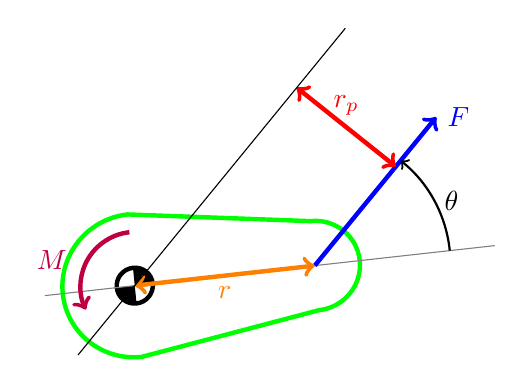
\begin{tikzpicture}[x={(0.9in,0.1in)},y={(-0.1,0.9in)}]

%\draw[blue, ultra thick] (0,0)--(0,2)--(2,2)--(2,0)--cycle;
\draw[ultra thick] (0,0) circle (0.1);
\fill[black] (0,0.1)--(0,0)--(0.1,0) arc[start angle=0, end angle=90, radius=0.1]--cycle;
\fill[black] (0,-0.1)--(0,0)--(-0.1,0) arc[start angle=180, end angle=270, radius=0.1]--cycle;

\draw[ultra thick, green] 
(0,0.4)--
(1,0.25) arc[start angle=90, end angle=-90, radius=0.25]--
(1,-0.25)--
(0,-0.4) arc[start angle=270, end angle=90, radius=0.4]--cycle;

\draw[thin, gray] (-0.5,0)--(2.0,0);

\draw[ultra thick, blue, ->] (1,0) -- (1.75,0.75) node[right]{$F$};
\draw[ultra thick, orange, <->] (0,0) -- (1,0) node[pos=0.5,below]{$r$};

\draw[ultra thick, red, <->] (1.0,1.0) -- (1.5,0.5) node[pos=0.5,above]{$r_p$};
\draw[thin, black] (-0.35, -0.35)--(1.3,1.3);

\draw[thick, black, ->] (1.75,0) arc[start angle=0, end angle=45, radius=0.75] node[pos=0.5, right] {$\theta$};

\draw[ultra thick, purple, ->] (0,0.3) arc[start angle=90, end angle=200, radius=0.3] node[pos=0.5, left] {$M\mbox{     }$};

\end{tikzpicture}

\begin{example}
\begin{outline}
\1 Newton-Meters ($N\mbox{-}m$)
\1 Foot-Pounds ($ft\mbox{-}lbf$)
\1 Ounce-Inches ($oz\mbox{-}in$)
\end{outline}
\end{example}

Moments produce angular accleration $\alpha$ inversely proportional to the 'moment of inertia' $I$ (sometimes abbreviated MOI)

\begin{equation}
	M_{CG} = I_{CG} \alpha
\end{equation}

The moment of inertia can be taken about anywhere, but taking it about the center of gravity (CG) makes things easier. The more mass, and the more it is spread out from the center, the higher the MOI.

\begin{example}
Moment of inertia of a flywheel
\begin{equation}
	I_{CG, solid disk} = \frac{m r^2}{2}
\end{equation}
\end{example}

\end{document}